\chapter{Teori}
I dette afsnit vil teorien, der ligger til grund for programmet, blive beskrevet, hvorunder tre hovedafsnit findes. Grafteori vil være det første afsnit, efterfulgt af vektorteori og  positionsbestemmelse. Under grafteori vil et par forskellige algoritmer tages i brug, hvoraf den bedste match til programmet findes. I grafteorien vil Nearest neighbour, Dijkstra’s algoritme og Double Minimum Spanning Tree algoritmerne blive beskrevet. I vektorteorien vil teorien bag udregning af afstanden mellem to knuder, eller en knude og en rute gøres rede for. Denne teori vil blive brugt i programmet til dannelse af rute, og udregning af nærliggende attraktioner.

\section{Grafteori}
Grafteori er et afsnit i denne rapport, som omhandler en generel forklaring på grafteori, hvorefter teorien bag Nearest neighbour algoritmen, Dijkstra’s algoritmen, Double Minimum Spanning Tree og Traveling salesman problem vil blive beskrevet. Alt dette beskrives, for at give et udgangspunkt for implementering af en hensigtsmæssig algoritme i programmet for denne rapport.

\subsection{Begrebsbeskrivelse}
En knude er et punkt på grafen. Knuder vil i denen rapports sammenhæng være attraktioner. \newline
En kant forbinder to knuder. Kanter kan vægtes, i denne rapport vil vægtningen af kanter være afstanden mellem de to knuder som kanten forbinder. \newline
En path er en rute gennem et antal knuder, hvor startknuden ikke er endeknuden. \newline
Et circuit er en rute gennem et antal knuder, hvor startknuden også er endeknuden. \newline
Et  Hamiltonian circuit er et circuit, hvori alle knuder er besøgt én gang, med undtagelse af slutpunktet, som skal være det samme som startpunktet. \newline
I denne rapport søges et circuit, som går igennem alle knuder én gang, hvor en samlet vægtning af kanterne (længden af ruten) bliver så kort som mulig. Dette er i grafteori også kaldet Traveling salesman problem. En umiddelbar løsning til TSP ville ville være at undersøge alle mulige Hamiltonian circuits, og finde den korteste. Problemet er, at når en graf med n knuder skal undersøges, skal der bruges (n–1)!/2 udregninger. Dette skyldes, at efter en startknude er valgt, vil der være (n – 1) mulige knuder som næste punkt, og derefter (n – 2) osv. Da der ikke er en bestemt retning på Hamiltonian circuits, vil der altid være to veje, hvor den ene beskriver den anden  bare omvendt. Derfor fås (n – 1)!/2. 
Med 25 knuder vil der være (24)!/2, som svarer til \[3.1 * 10^{23}\] forskellige Hamiltonian circuits. Hvis det antages, at det tager et nanosekund at udregne ét Hamiltonian circuit, vil dette tage cirka 10 millioner år, at udregne alle circuits, og finde den optimale. Derfor bruges algoritmer, som udregner en løsning som er tæt på den optimale. Nedenfor vil tre sådanne algoritmer blive beskrevet. \citep{DisMat}

\subsection{Nearest neighbour algoritmen}
\begin{wrapfigure}{}{0.4\textwidth}
	\vspace{70pt}
	\begin{center}
		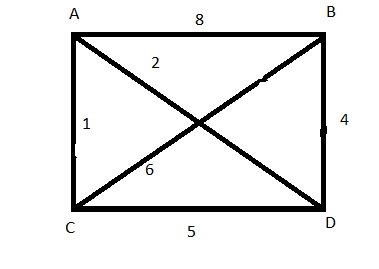
\includegraphics[scale=0.8]{grafteori2} \newline
		\textit{ Figur 5.1: Hamiltonian Circuit. \newline Følger kanter med laveste værdier.}
	\end{center}
	\vspace{-10pt}
\end{wrapfigure}
Fremgangsmetode: \newline
Vælg en startknude. \newline
Følg kanten med den laveste vægtning. \newline
Check om der er flere ubesøgte knuder tilbage, hvis ja, gå tilbage til trin 2. \newline
Gå tilbage til startknuden. \newline
Fra den knude der behandles, skal kanten med den laveste værdi følges. Hvis alle knuder er besøgt, skal kanten der går tilbage til startknuden vælges. \newline
Eksempelvis i dette tilfælde (figur 5.1),  er den endelige rutes længde, udregnet med NNA: 1+5+4+8+2 = 20. \newline
NNA udregner ikke med sikkerhed en optimal rute, hvilket skyldes at den ikke tager højde for konsekvenserne af de skridt den tager. Selvom det første skridt er det korteste blandt de mulige, kan det i det lange løb godt ende med at blive en meget længere rute der bliver sammensat. En måde dette kan optimiseres, er ved at køre NNA flere gange med forskellige startpunkter. Her kaldet en udvidet NNA. Nedenfor er en udvidet NNA beskrevet. \newline
Fremgangsmetode: \newline
Udfør NNA på en ny ikke testet startknude. \newline
Er der knuder der ikke er testet som startknude, hvis ja, gå tilbage til trin 1. \newline
Vælg det korteste circuit af de testede. \newline


\begin{tabular}{| l | l | l | l | l | l |}
	\hline
	& A & B & C & D  \\ \hline
	A & - & 8 & 1 & 2 \\ \hline
	B & 8 & - & 6 & 3  \\ \hline
	C & 1 & 6 & - & 5  \\ \hline
	D & 2 & 4 & 5 & -  \\ \hline
	\hline
\end{tabular}\newline

De mulige ruter er: \newline
ACDBA = 1 + 5 + 4 + 8 = 18\newline
BDACB = 4 + 2 + 1 + 6 = 13\newline
CADBC = 1 + 2 + 4 + 6 = 13\newline
DACBD = 2 + 1 + 6 + 4 = 13\newline
Den korteste rute er altså BDACB, hvilket er 5 kortere end den antagede rute. Den optimale circuit fundet med udvidet NNA er derfor denne rute. Dette tager standard NNA ikke højde for, da den starter i en valgt start-knude, og derefter følger kanten, med den derfra laveste værdi. NNA kræver ikke lige så mange beregninger som en brute force udregning kræver, og kan derfor bruges i praksis, dog er den ikke sikker på at finde den optimale rute.


\subsection{Dijkstra's algoritme}
Udover NNA, findes også Dijkstra’s algoritme, hvor første trin er, at bestemme ende-knuden, og sætte dens distance til nul. Denne knude sættes til at være den første knude, som behandles. I det en knude er checket færdig, vil denne knude markeres som ”besøgt”, og kanten med den mindste værdi følges, og næste knude markeres som ”nuværende” knude. En kant bliver kun fulgt, hvis det er den korteste rute, tilregnet tidligere kanter.
Problematikken med Dijkstra’s algoritme i forhold til dette projekt er, at den checker den korteste rute fra start-knude til slut-knude, men den indkluderer ikke nødvendigvis alle knuder som oplyses. I det denne rapport er afgrænset til fugleflugtslinjer, vil Dijkstra’s ikke være den optimale. Hvis en rute igennem en by, hvor der er tilregnet veje, stier og andre knuder, vil Dijkstra’s være det bedste valg. Denne algoritme vil også være i brug ved den optimale løsning. Ved brug af Dijkstra’s algoritme, vil den nuværende rute altid blive testet for, hvorvidt ruten der undersøges efter, er kortere eller længere end den hidtil korteste rute. Hvis den er kortere, vil denne rute blive sat som den hidtil korteste rute. \citep{Dijkstra}

/subsection{Double Minimum Spanning Tree}
Double Minimum Spanning Tree er algoritmen der ligger til grund for Christofides algoritme, hvor DMST har tre trin: \newline
Først oprettes et minimum spanning tree, som indkluderer alle knuder. \newline
Alle kanter duplikeres. \newline
Den korteste rute findes mellem disse kanter, hvor en knude kun besøges én gang. \newline
Hvis der ikke er kanter til ubesøgte knuder, oprettes en ”genvej” fra den nuværende knude til en ubesøgt knude \citep{DMST}. \newline
Et minimum spanning tree findes ved at tage så få kanter som muligt, med den laveste vægtning, så alle knuder er besøgt blot én gang.

\subsection{Opsummering}
Da dette projekt forholder sig til en forholdvis kort rute, men hovedsagligt tager udgangspunkt i en rute hvortil der kan tilføjes flere punkter, for at lave en interessant rute, er NNA valgt som den bedste kandidat. Dette skyldes, at Dijkstra’s ikke nødvendigvis indkluderer alle knuder, da den finder en kort rute fra startpunkt til slutpunkt. DMST finder en mere optimal rute end NNA, men samtidig kræver den længere tid at udregne, og derfor blev NNA valgt som den optimale algoritme til dette projekt.

\section{Vektorteori}

\begin{wrapfigure}{}{0.4\textwidth}
	\vspace{-10pt}
	\begin{center}
		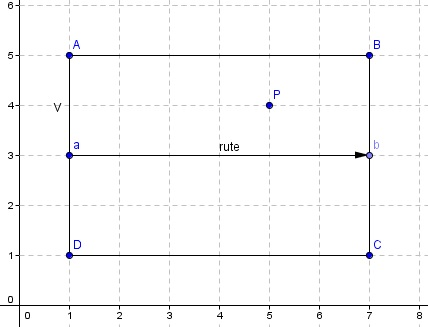
\includegraphics[scale=0.6]{matematikteori1} \newline
		\textit{Figur 5.2: Eksempel på om en attraktion er indenfor punkt a og b.}\newline
	\end{center}
	\vspace{-40pt}
\end{wrapfigure}

Essensen i dette projekt er at finde en flerpunktsrute mellem nogle valgte attraktioner, hvor brugeren skal have mulighed for, at vælge nogle attraktioner til deres rute. Gruppen vil ikke diktere hvad en interessant rute er for brugeren, derfor skal de have muligheden for at vælge de foreslåede attraktioner til eller fra.

Der tages nu udgangspunkt i figur 5.2. En del af brugerens rute ligger fra attraktion a til attraktion b. Der skal nu tjekkes om der ligger andre attraktioner mellem afstanden fra a til b (eller AB), og med bredden AD hvor brugeren vil blive spurgt om denne attraktion skal tilføjes til ruten. AD er i projektets program sat til at være V * 2. Dette vil blive udregnet vha. vektorer 
Hvis der antages at punktet P er en attraktion som programmet skal tjekke, ligger denne inden for længden af ruten AB og bredden AD. Dette tjekkes med følgende formel:
\[0 < AP \cdot AB < AB \cdot AB \wedge 0 < AP \cdot AD < AD \cdot AD \]
Hvor prikproduktet af vektorerne AP og AB, skal være større end 0 og mindre end prikproduktet af vektorerne AB og AB. Det samme vil gælde for AD i stedet for AB.

Lad nu som om det de informationer der kendes er punkterne a og b, samt længden på vektor ab som vil være 6 og vektoren vil hedde:
\[ \begin{bmatrix} 6 \\ 0 \end{bmatrix} \]

Først ønskes punktet A findes, som gøres ved først at finde tværvektoren. Tværvektoren findes ved at bytte 1. og 2. koordinat rund og ændre fortegn på første koordinaten:
\[ \begin{matrix} a1 \\ a2 \end{matrix} = \begin{matrix} -a2 \\ a1 \end{matrix} \]
Tværvektoren hedder: 
\[ \begin{bmatrix} 6 \\ 0 \end{bmatrix} \text{ ,} \]
og har udgangs punkt fra punktet a. \newline
I dette eksempel skal der søges efter ekstra attraktioner langs ruten, svarende til 1/3 af rutens længde. Så for at finde koordinaterne til punktet A, finder vi først en enhedsvektor for tværvektoren, dette gøres med formlen:
\[ \overrightarrow{e} = \frac{1}{\overrightarrow{a}}*\overrightarrow{a} \] 

Dette giver en vektor: 
\[\ \begin{bmatrix} 0 \\ 1 \end{bmatrix} \text{ ,} \]
som også har udgangspunkt fra punktet a. Som tidligere nævnt søges der efter ekstra attraktioner langs ruten, svarende til 1/3 af rutens længde, så enhedsvektoren multipliceres med to, hvilket giver en vektor: 
\[\ \begin{bmatrix} 0 \\ 2 \end{bmatrix} \textbf{ .} \]
Denne vektor lægges til koordinaterne til punktet a, hvilket vil give punktet:
\[\ A = \begin{bmatrix} 1 \\ 3 \end{bmatrix} + \begin{bmatrix} 0 \\ 2 \end{bmatrix} = \begin{bmatrix} 1 \\ 5 \end{bmatrix} \text{ .} \]

Punktet D vil så ledes findes  ved at tage vektoren fra før og multiplicere med -2 og lægge punktet A til:
\[\ D = \begin{bmatrix} 0 \\ 2 \end{bmatrix} * -2 = \begin{bmatrix} 0 \\ -4 \end{bmatrix} + \begin{bmatrix} 1 \\ 5 \end{bmatrix} = \begin{bmatrix} 1 \\ 1 \end{bmatrix} \text{ .} \]


Dog vil der først findes en vektor AP mellem punkterne A og P med formlen: \[ \overrightarrow{AP} = \begin{matrix}X2-X1 \\ Y2-Y1\end{matrix} \]
Vektor AP: A(1,5) og P(5,4): \[ \overrightarrow{AP} = \begin{bmatrix}5-1 \\ 4-5\end{bmatrix} = \begin{bmatrix} 4 \\ -1 \end{bmatrix} \]
\[ \text{Vektor AB er allerede kendt, da det er det samme som } \overrightarrow{ab} \text{.} \]
For at projektere AP på AB skal følgende formel benyttes: \citep{ProjektionAfVektor} \[ b_{a} = (\frac{a*b}{|a|^2}) * a \]
Med denne formel vil vektoren b blive projekteret på vektoren a. I tælleren findes prikproduktet som kan findes ved at: \[ a \cdot b = \begin{matrix}X1 * X2 \\ Y1 * Y2\end{matrix}  \]
I nævneren findes længden på vektor a i anden, som kan regnes ved at sige: \[ \sqrt{ax^2+ay^2}^2 \]
Hvis der forsat tages udgangspunkt i eksemplet med figur 5.2, vil projektionen af AP på AB kunne ses på figur 5.3:

\begin{wrapfigure}{r}{0.4\textwidth}
	\vspace{-20pt}
	\begin{center}
		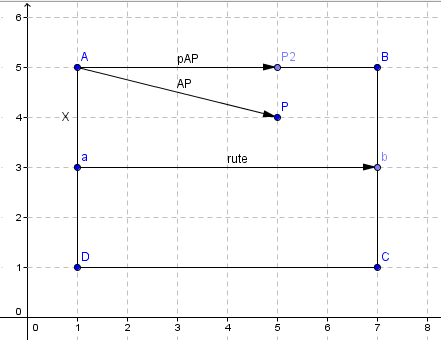
\includegraphics[scale=0.6]{matematikteori2} \newline
		\textit{Figur 5.3: Fortsat eksempel på om en attraktion er indenfor punkt a og b.}\newline
	\end{center}
	\vspace{-20pt}
\end{wrapfigure}

Prikproduktet af vektorerne: \[ \overrightarrow{AP} \cdot \overrightarrow{AB} = \begin{bmatrix} 4 & 6 \\ -1 & 0 \end{bmatrix} = 4*6+(-1)*0 = 24 \]
Længden af AB opløftet i anden vil være: \[ \sqrt{6^2+0^2}^2 = 36 \]
Ud fra dette kan vektoren fra projektionen af AP på AB findes: 
\[ \frac{24}{36} * \begin{bmatrix} 6 \\ 0 \end{bmatrix} \rightarrow \frac{24}{36} * 6 \wedge \frac{24}{36} * 0 = \begin{bmatrix} 4 \\ 0 \end{bmatrix} \]
Hvor resultatet vil give en ny vektor: \[ \begin{bmatrix} 4 \\ 0 \end{bmatrix} \text{ ,} \] 
som også vil have startpunkt i A. Hvis der igen tages udgangspunkt i formlen:\newline
\[0 < AP \cdot AB < AB \cdot AB \wedge 0 < AP \cdot AD < AD \cdot AD \]
overholder punktet P første del, og ovenstående metode skal derfor gentages med vektoren AD i stedet for AB, for matematisk at finde ud af om punktet ligger inden 	for den afsatte bredde og længden af ruten a til b. Ved udregning af projektionen af AP på AD vil den nye vektor hedde: \[ \begin{bmatrix} 0 \\ -1 \end{bmatrix} \text{ .} \]\newline
\textbf{Opsummering}\newline
I grafteorien blev der konkluderet, at Nearest Neighbor algoritmen er den mest egnede til programmet, da dette projekt forholder sig til udregning af en relativt kort rute, hvorved en interessant rute kan findes efterfølgende. Vektorteorien gjorde grund for udregning af, hvilke attraktioner der er nærliggende, så en interessant rute kan findes ud fra ruten der i første omgang bliver dannet af NNA.

\section{Positionsbestemmelse}
\begin{wrapfigure}{r}{0.4\textwidth}
	\vspace{-20pt}
	\begin{center}
		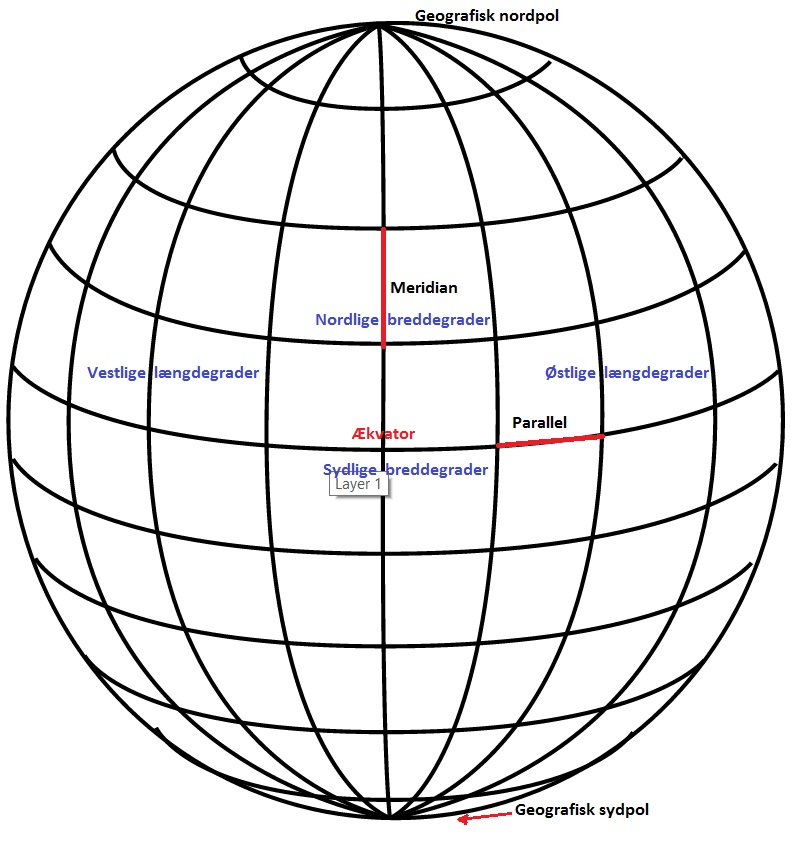
\includegraphics[scale=0.3]{globerapport} \newline
		\textit{Figur 5.4: Fortsat eksempel på om en attraktion er indenfor punkt a og b.}\newline
	\end{center}
	\vspace{-30pt}
\end{wrapfigure}
I projektet bruges længde- og breddegrader til at udregne afstanden mellem attraktionerne. Dette sker kort sagt ved, at finde to koordinatsæt og bruge pythagoras’ sætning til at udregne afstanden. I dette afsnit vil der være en kort forklaring om længde- og breddegrader, og hvordan gruppen har brugt dem i dette projekt.\newline
Længdegrader er de lodrette streger der kan ses på globussen i figur X. De lodrette streger kaldes for en meridian, hvor disse vil have mindre afstand mellem hinanden i nærheden af de geografiske poler, i forhold til når de er tæt ved ækvator. De vandrette streger er breddegrader, hvor disse er kaldt paralleller. Breddegradernes afstand ændre sig ikke på samme måde som længdegraderne. \citep{PM} \newline
Ligesom på en cirkel er jorden delt op i 360 længdegrader. 0 grader vil ligge i observatoriet i Greenwich, som ligger i London området. De 360 grader er opdelt i 180 vestlige og 180 østlige længdegrader. Breddegrader begynder fra 0 grader ved ækvator og rammer 90 grader ved en af polerne, i henholdsvis nordlige- eller sydlige breddegrader. \citep{PM}\newline
Der findes forskellige metoder til at notere koordinatsættet i form af længde- og breddegrader. I dette projekt bruges der et grade tal med decimaler, eksempelvis 57,12345. I dette system nævnes ikke om det er i sydlig, nordlig,vestlig eller østlig retning, men istedet er de sydlige breddegrader og vestlige længdegrader, negative tal . En anden måde at notere dette er at dele det op i grader, minutter og sekunder, hvor der går 60 sekunder på et minut og 60 minutter på en grad. Breddegraderne ligger fast på ca. 111 km pr. grad, mens længdegraderne variere da der bliver kortere afstand mellem meridianerne desto tættere de er på polerne. Med andre ord kan det siges, at hvis en person er på 5. længdegrad, så er personen 5 længdegrader fra Greenwich (0 grader), men afstanden i km for hver længdegrad ændre sig i forhold til hvilken breddegrad der undersøges. Denne afstand kan enten udregnes eller findes i en tabel. I dette projekt er det afstanden slået op i en tabel \citep{Earth}. Som viser at der ved Aalborg, ved den 57. breddegrad, går 1012.87 meter per minut, altså 1012.87*60 =  60772.2 meter pr grad = 60.77 kilometer pr grad. \citep{PM}
